\chapter{Evaluating the Impact of Constraints on Feature-Selection Results}
\label{sec:syn}

\section{Overview}
\label{sec:syn:overview}

\paragraph{Scope}

Building on the motivation provided in Section~\ref{sec:introduction:research-gaps}, this chapter lays the foundations for constrained feature selection in general.
In contrast, the subsequent three chapters will focus on specific constraint types.
Besides formally introducing constrained feature selection, this chapter empirically evaluates the impact of constraints.
Generally, adding constraints may lower feature-set quality.
An important question is if there are sweet spots, i.e., high-quality feature sets that satisfy the constraints.

\paragraph{Contributions}

Our contribution in this chapter is twofold:

(1) We formalize constrained feature selection as an optimization problem and discuss how to solve it.
Our problem definition is independent of the feature-selection method.

(2) We conduct a systematic, domain-independent study to analyze the impact of constraints on feature-selection results.
To this end, we propose an experimental design that enables such an analysis.
In particular, we use 35 regression datasets from various domains and generate random constraints systematically.
We vary the constraint types, number of constraints, and features used.
Further, we define evaluation metrics that quantify the constraints and the feature-selection results.
We then empirically evaluate the relationships between these metrics.
We find optimal feature sets with a Satisfiability Modulo Theories (SMT) solver, which supports a broad range of constraint types.
In particular, we use univariate filter feature selection as the objective and formulate constraints in propositional logic and linear arithmetic.
Section~\ref{sec:syn:evaluation:summary} summarizes key results.

\paragraph{Materials}

We publish all our code and experimental data online (cf.~Section~\ref{sec:introduction:materials}).

\paragraph{Prior works}

The content of this chapter bases on the following prior work:
%
\begin{itemize}
	\item \fullcite{bach2022empirical}
\end{itemize}

\paragraph{Chapter outline}

The remainder of this chapter is structured as follows:
Section~\ref{sec:syn:approach} describes and analyzes constrained feature selection.
Section~\ref{sec:syn:experimental-design} outlines our experimental design.
Section~\ref{sec:syn:evaluation} presents the corresponding experimental results.

\section{Constrained Feature Selection}
\label{sec:syn:approach}

In this section, we introduce the problem of constrained feature selection.
After briefly defining the overall optimization problem (cf.~Section~\ref{sec:syn:approach:problem}), we describe potential constraints (cf.~Section~\ref{sec:syn:approach:constraints}) and how to consider them (cf.~Section~\ref{sec:syn:approach:optimization}).
Finally, we discuss the time complexity of this problem (cf.~Section~\ref{sec:syn:approach:complexity}).

\subsection{Optimization Problem}
\label{sec:syn:approach:problem}

For constrained feature selection, we keep the objective and decision variables of conventional feature selection (cf.~Definition~\ref{def:fs:feature-selection}).
I.e., we still optimize the feature-set quality~$Q(s,X,y)$ for a dataset~$X \in \mathbb{R}^{m \times n}$ and a prediction target~$y \in Y^m$ by making feature-selection decisions~$s \in \{0, 1\}^n$.
Thus, the general concept of constrained feature selection is independent of the feature-selection method, which determines the objective~$Q(s,X,y)$.
The novelty is admitting a set~$C$ of user-defined constraints for this optimization problem.
Each constraint $c \in C$ maps the feature-selection decisions~$s$ to true (1) or false (0).
We assume hard constraints, i.e., a valid feature set needs to satisfy all constraints:
%
\begin{equation}
	\begin{aligned}
		\max_s &\quad Q(s,X,y) \\
		\text{subject to:} &\quad \forall c \in C:~ c(s) = 1 \\
		\text{with:} &\quad C \subseteq \{c \mid c: \{0,1\}^n \to \{0, 1\}\}
	\end{aligned}
	\label{eq:syn:cfs-problem}
\end{equation}
%
The full textual problem definition corresponding to Equation~\ref{eq:syn:cfs-problem} is the following:
%
\begin{definition}[Constrained feature selection]
	Given a dataset~$X \in \mathbb{R}^{m \times n}$ with prediction target~$y \in Y^m$, and a set of constraints $C \subseteq \{c \mid c: \{0,1\}^n \to \{0, 1\}\}$,
	\emph{constrained feature selection} is the problem of making feature-selection decisions~$s \in \{0,1\}^n$ that maximize a given notion of feature-set quality~$Q(s,X,y)$ while satisfying all constraints, i.e., ${\forall c \in C:}~ c(s) = 1$.
	\label{def:syn:constrained-feature-selection}
\end{definition}

\subsection{Constraints}
\label{sec:syn:approach:constraints}

There is a broad range of possible constraint types.
Limiting the feature-set size to a user-defined cardinality~$k \in \mathbb{N}$, as common in many existing feature-selection methods, is only one possible constraint type.
In general, users should ultimately decide which constraint types to employ.
However, depending on the optimization method (cf.~Section~\ref{sec:syn:approach:optimization}), it makes sense to limit the categories of admissible constraint types, e.g., by prescribing particular logics to formulate constraints.
Such a limitation still offers more flexibility than only allowing one particular constraint type, as common in related work (cf.~Section~\ref{sec:related-work:constraints:feature-selection}).
In our work, we admit arbitrary constraints in propositional logic and linear arithmetic.
These two categories are domain-independent and allow the formulation of various expressive constraint types.
In particular, all constraint types in our domain-specific case study (cf.~Chapter~\ref{sec:ms}) can be formulated that way.
Additionally, propositional logic and linear arithmetic subsume typical constraint types from related work (cf.~Chapter~\ref{sec:related-work:constraints}).
Finally, these logics allow using a white-box solver for optimization (cf.~Section~\ref{sec:syn:approach:optimization}).

\paragraph{Propositional constraints}

Propositional constraints describe relationships between features with propositional logic.
The binary selection decisions $s_j \in \{0,1\}$ correspond to the logical values $\{\text{false}, \text{true}\}$.
One can now use logical operators like AND~($\land$), inclusive OR~($\lor$), exclusive OR~($\oplus$), NOT~($\lnot$), IMPLIES~($\rightarrow$), and IFF~($\leftrightarrow$).
For example, $s_1 \rightarrow s_2$ means that if Feature~1 is selected, then Feature~2 has to be selected as well.
By combining the operators, one can describe more complex relationships.
For example, $(s_4 \land s_7 \land s_{10}) \oplus (s_2 \land s_{11})$ means that either the three features from the first group or the two features from the second group have to be selected.

\paragraph{Arithmetic constraints}

The theory of linear arithmetic supports four operators~\cite{barrett2018satisfiability}:
addition~($+$), subtraction~($-$), multiplication~($\cdot$), and less-or-equal~($\leq$).
In the terminology of first-order logic, the first three operators are functions, returning another arithmetic value, while the inequality is a predicate, yielding a logical value.
Linear arithmetic does not allow multiplying two variables, as at least one operand has to be a constant~\cite{barrett2018satisfiability}.
In general, one can use linear-arithmetic constraints by assigning each feature a numeric value and formulating an inequality.
For example, suppose that each feature has a weight~$w_j \in \mathbb{R}_{\geq 0}$, e.g., measurement cost, and one wants to select a feature set with a total weight below a threshold $w_{\text{max}} \in \mathbb{R}_{> 0}$.
This yields the following linear inequality: 
%
\begin{equation}
	\sum_{j=1}^n s_j \cdot w_j \leq w_{\text{max}}
\end{equation}

For instance, such a situation occurs if feature values are obtained with sensors with different energy consumption, and the total amount of energy per measurement is limited.

A cardinality constraint on the feature-set size is a special case of a weighted-sum constraint.
It has uniform weights and a desired minimum, exact, or maximum cardinality~$k \in \mathbb{N}$:
%
\begin{equation}
	\sum_{j=1}^n s_j = k
	\label{eq:syn:cardinality}
\end{equation}

One may use propositional and arithmetic constraints interchangeably in some situations.
Think of a group of five features, and one wants to select at least one of them.
Arithmetically, the sum of selection decisions for these five features should be at least one.
With propositional logic, one may employ the OR~($\lor$) operator.

\subsection{Optimization Methods}
\label{sec:syn:approach:optimization}

Depending on the formulation of the constrained optimization problem, different optimization methods are suitable.
Conventional feature-selection methods are typically not designed to operate in a constrained search space; they support a cardinality constraint at most.
Adapting individual feature-selection methods to individual constraint types is feasible in some cases but lacks generality.
Instead, we propose to use a generic white-box or black-box optimizer to tackle constrained feature selection.

White-box optimizers consider the internal structure of the optimization problem.
In particular, they must support formulating the chosen objective and constraint types.
Nevertheless, they provide more flexibility than adapting existing feature-selection methods since they typically support a broad range of expressions.
In particular, they allow users to combine arbitrary constraints within the supported logic declaratively.

In contrast, black-box optimization methods only process the objective value without knowing how its function is defined.
This characteristic increases generality but also means that some information about the internals of the optimization problem remains unused.
In some cases, constraint types may be black-box functions as well.

Our chapter on alternative feature selection (cf.~Section~\ref{sec:afs:approach:objectives}) provides a detailed discussion on white-box and black-box optimization for different feature-selection methods.
In the current chapter's experiments, we use univariate filter feature selection (cf.~Equation~\ref{eq:fs:univariate-filter}) as the optimization objective.
This simple linear objective is independent of the prediction model and allows us to use an off-the-shelf white-box solver to find optimal feature sets.
In particular, we employ a Satisfiability Modulo Theories (SMT) optimizer~\cite{barrett2018satisfiability}.
Such solvers support constraints in propositional logic and first-order theories like arithmetic, bit vectors, or arrays.
We already decided to formulate constraints in propositional logic and linear arithmetic (cf.~Section~\ref{sec:syn:approach:constraints}), which fits the scope of SMT.
The objective function in Equation~\ref{eq:fs:univariate-filter} is also linear once the feature qualities~$q(X_{\cdot{}j},y)$ are computed.

If all constraints are in propositional logic, then the optimization problem with this objective becomes a weighted \textsc{Max One} problem~\cite{khanna1997complete}.
This is a special case of a weighted partial maximum satisfiability (\textsc{MaxSAT}) problem~\cite{bacchus2021maximum, li2021maxsat}, where the individual binary decision variables form the soft clauses for optimization and the user-defined constraints constitute the hard clauses.
Such a problem formulation gives way to specialized \textsc{MaxSAT} solvers.
If we include arithmetic constraints, the formulation is a \textsc{MaxSMT} problem~\cite{nieuwenhuis2006sat}.

\subsection{Time Complexity}
\label{sec:syn:approach:complexity}

We analyze three aspects of time complexity for constrained feature selection:
the size of the search space for exhaustive search, parameterized complexity, and $\mathcal{NP}$-hardness.
While the results here are relatively straightforward, they also lay the foundation for further complexity analyses regarding alternative feature selection (cf.~Section~\ref{sec:afs:approach:complexity}) and constrained subgroup discovery (cf.~Sections~\ref{sec:csd:approach:cardinality:complexity} and~\ref{sec:csd:approach:alternatives:complexity}).

\paragraph{Exhaustive search}

Without constraints, the search space of feature selection grows exponentially with the number of features~$n$.
In particular, there are $2^n - 1$ possibilities to form a non-empty feature set of arbitrary size.
In the worst case, finding the optimal feature set requires iterating over this entire space.
In practice, particular notions of feature-set quality may allow finding the optimum faster, or a feature-selection method may only strive for an approximate solution.

Constraints can reduce the search space, but the upper bound remains the same:
%
\begin{proposition}[Complexity of exhaustive search for (constrained) feature selection]
	An exhaustive search for feature selection with or without constraints (cf.~Definitions~\ref{def:fs:feature-selection} and~\ref{def:syn:constrained-feature-selection}) needs to evaluate $O(2^n)$ feature sets.
	\label{prop:syn:complexity-constrained-exhaustive}
\end{proposition}
%
Even if constraints reduce the search space, an essential question is whether one can efficiently enumerate all valid feature sets.
The latter is possible for cardinality constraints, which have $\binom{n}{k} = \frac{n!}{k! \cdot (n-k)!} \leq n^k$ solution candidates for a fixed feature-set size~$k$:
%
\begin{proposition}[Complexity of exhaustive search for feature selection with cardinality constraint]
	An exhaustive search for feature selection (cf.~Definition~\ref{def:fs:feature-selection}) with an exact cardinality constraint (cf.~Equation~\ref{eq:syn:cardinality}) needs to evaluate~$O(n^k)$ feature sets.
	\label{prop:syn:complexity-cardinality-exhaustive}
\end{proposition}

\paragraph{Parameterized complexity}

Depending on the constraint types employed, the size of the search space may no longer be exponential in~$n$ but may depend on other parameters.
This situation occurs for cardinality constraints:
If we assume $k \ll n,~k \in O(1)$, i.e., $k$ being a small constant, independent from~$n$, then the complexity in Proposition~\ref{prop:syn:complexity-cardinality-exhaustive} is polynomial in~$n$.
This assumption makes sense if one wants to obtain a small feature set from a high-dimensional dataset, which is a typical goal of feature selection.
However, the exponent~$k$ may still render an exhaustive search practically infeasible.
In terms of parameterized complexity, the problem resides in class~$\mathcal{XP}$ since the complexity term has the form $O(f(k) \cdot n^{g(k)})$~\cite{downey1997parameterized}, here with parameter~$k$ and functions $f(k) = 1$, $g(k) = k$.
%
\begin{proposition}[Parameterized complexity of feature selection with cardinality constraint]
	The problem of feature selection (cf.~Definition~\ref{def:fs:feature-selection}) with an exact cardinality constraint (cf.~Equation~\ref{eq:syn:cardinality}) resides in the parameterized complexity class~$\mathcal{XP}$ for the parameter~$k$.
	\label{prop:syn:complexity-cardinality-xp}
\end{proposition}

\paragraph{NP-Hardness}

The constraint types also influence whether constrained feature selection resides in complexity class $\mathcal{P}$ or $\mathcal{NP}$.
In general, even determining whether there is at least one valid solution candidate is $\mathcal{NP}$-hard for propositional logic~\cite{cook1971complexity} and SMT~\cite{barrett2018satisfiability}.
In particular, only a few categories of propositional formulas guarantee a polynomial-time check for satisfiability~\cite{schaefer1978complexity}.
Further, optimization problems are generally at least as hard as the corresponding decision problems~\cite{garey2003computers}.
Thus, we obtain the following proposition:
%
\begin{proposition}[Complexity of constrained feature selection with propositional constraints]
	Assuming an arbitrary feature-set quality function~$Q(s,X,y)$ whose value can be computed in polynomial time,
	the problem of constrained feature selection (cf.~Definition~\ref{def:syn:constrained-feature-selection}) with arbitrary constraints in propositional logic is $\mathcal{NP}$-complete.
	\label{prop:syn:complexity-constrained-np}
\end{proposition}
%
This result is not tied to a particular feature-selection method.
Even with a univariate objective (cf.~Equation~\ref{eq:fs:univariate-filter}) and propositional constraints, optimization is hard in general:
%
\begin{proposition}[Complexity of constrained feature selection with univariate objective and propositional constraints]
	Assuming univariate feature qualities (cf.~Equation~\ref{eq:fs:univariate-filter}),
	the problem of constrained feature selection (cf.~Definition~\ref{def:syn:constrained-feature-selection}) with arbitrary constraints in propositional logic is $\mathcal{NP}$-complete.
	\label{prop:syn:complexity-constrained-univariate-np}
\end{proposition}
%
In particular, this weighted \textsc{Max One} problem only resides in $\mathcal{P}$ for a few categories of constraint types, but in $\mathcal{NP}$ for all others, and even finding an approximate solution with guaranteed quality may be hard~\cite{khanna1997complete}.
One polynomial-time case concerns the cardinality constraint.
If the optimization problem only involves this constraint type, one can sort the univariate feature qualities and pick the $k$ highest ones to obtain the exact optimum:
%
\begin{proposition}[Complexity of feature selection with univariate objective and cardinality constraint]
	Assuming univariate feature qualities (cf.~Equation~\ref{eq:fs:univariate-filter}),
	the problem of feature selection (cf.~Definition~\ref{def:fs:feature-selection}) with an exact cardinality constraint (cf.~Equation~\ref{eq:syn:cardinality}) has a time complexity of $O(n \cdot \log n)$.
	\label{prop:syn:complexity-cardinality-univariate-np}
\end{proposition}

\section{Experimental Design}
\label{sec:syn:experimental-design}

In this section, we introduce our experimental design for studying the impact of constraints.
We start with a brief overview (cf.~Section~\ref{sec:syn:experimental-design:overview}).
Next, we describe the components of the experimental design: constraints (cf.~Section~\ref{sec:syn:experimental-design:constraints}), objective function (cf.~Section~\ref{sec:syn:experimental-design:objective}), prediction models (cf.~Section~\ref{sec:syn:experimental-design:prediction}), evaluation metrics (cf.~Section~\ref{sec:syn:experimental-design:metrics}), and datasets (cf.~Section~\ref{sec:syn:experimental-design:datasets}).
Finally, we briefly outline our implementation (cf.~Section~\ref{sec:syn:experimental-design:implementation}).

\subsection{Overview}
\label{sec:syn:experimental-design:overview}

We evaluate the impact of constraints on feature-selection results with 35 regression datasets.
For our analyses, we repeatedly generate random constraints of ten different types and optimize the objective of univariate filter feature selection.
We use four evaluation metrics to quantify constraints and three evaluation metrics to quantify feature-selection results.
We analyze how the evaluation metrics relate to each other and how the impact of constraints differs between constraint types.

\subsection{Constraints}
\label{sec:syn:experimental-design:constraints}

The space of potential constraints is vast.
To obtain general insights, we systematically generate constraints with many repetitions, varying three aspects.
First, the \emph{generation method} varies the features involved in constraints, i.e., the operands of the constraints.
Second, the \emph{constraint type} defines the operator for constraints, e.g., AND, OR, etc.
Third, we conduct 10-fold cross-validation on multiple datasets (cf.~Section~\ref{sec:syn:experimental-design:datasets}).

\begin{algorithm}[t]
	\DontPrintSemicolon
	\KwIn{
		Constraint type $t$, \newline
		Optimization problem $o$, \newline
		Number of iterations $\mathit{n\_iters} \in \mathbb{N}$
	}
	\KwOut{Evaluation metrics from Section~\ref{sec:syn:experimental-design:metrics}}
	\BlankLine
	\For{$\mathit{iters} \leftarrow 1$ \KwTo $\mathit{n\_iters}$}{
		$o' \leftarrow o$\tcp*[r]{make copy}
		$C \leftarrow \emptyset$\tcp*[r]{set of constraints}
		$\mathit{num}_{\text{co}} \leftarrow$ Choose $\mathit{num}_{\text{co}} \in \{1, \dots, 10\}$ uniformly random\; \label{al:syn:constraint-generation:line:num-constraints}
		\For{$\mathit{con\_iters} \leftarrow 1$ \KwTo $\mathit{num}_{\text{co}}$}{
			\If{$t$ is `single' constraint}{ \label{al:syn:constraint-generation:line:num-features-start}
				$n' \leftarrow 2$\tcp*[f]{number of features in constraint}
			}
			\ElseIf{$t$ is `group' constraint}{
				$n' \leftarrow$ Choose $n' \in \{2, \dots, n\}$ uniformly random\; \label{al:syn:constraint-generation:line:num-features-end}
			}
			$F \leftarrow $ Choose $n'$ distinct features uniformly random\; \label{al:syn:constraint-generation:line:choose-features}
			$c \leftarrow$ Apply $t$ to $F$\tcp*[r]{one constraint}
			$C \leftarrow C \cup \{c\}$\;
		}
		$o' \leftarrow$ Add $C$ to $o'$\;
		Solve $o'$\;
		Evaluate $o'$\;
	}
	\caption{Constraint-generation method for evaluating the constraints' impact.}
	\label{al:syn:constraint-generation}
\end{algorithm}

\paragraph{Generation method} 

We employ the same generation method for all constraint types except for two, which we discuss later.
The generation method varies several characteristics of a constraint set:
the number of constraints, the number of features in each constraint, and the actual features in each constraint.
This flexibility gives way to a broad coverage of the evaluation space but also causes considerable variance.
Consequently, we repeat the constraint generation $\mathit{n\_iters} = 1000$ times per combination of constraint type, dataset, and cross-validation split.
We call each iteration a \emph{constraint-generation run}.

Algorithm~\ref{al:syn:constraint-generation} outlines the process of generating and evaluating constraints.
The initial optimization problem $o$ only consists of the objective function (cf.~Section~\ref{sec:syn:experimental-design:objective}) initialized for the current cross-validation split and dataset.
In each constraint-generation run, we vary the number of constraints uniformly at random between one and ten (Line~\ref{al:syn:constraint-generation:line:num-constraints}).
Next, we decide on the number of features per constraint (Lines~\ref{al:syn:constraint-generation:line:num-features-start}--\ref{al:syn:constraint-generation:line:num-features-end}).
Our \emph{single} constraint types always involve two features, while \emph{group} constraint types support larger sets, with the group size $n' \in \{2, \dots, n\}$ chosen uniformly at random.
We choose the features involved in a constraint uniformly random as well, sampling without replacement (Line~\ref{al:syn:constraint-generation:line:choose-features}).
After creating the constraints, we add them to the optimization problem, run the optimizer, and compute the evaluation metrics (cf.~Section~\ref{sec:syn:experimental-design:metrics}).

\paragraph{Constraint types}

To specify constraint types, we can select from a broad range of possible operators.
Also, combining operators can yields further operators.
For example, NAND can be expressed with an AND and a NOT.
Thus, exhaustively evaluating all possible constraint types is infeasible.
Additionally, the datasets in this study (cf.~Section~\ref{sec:syn:experimental-design:datasets}) come from different domains.
Thus, it is impossible to formulate a common set of domain-specific constraints.
Instead, we use ten generic constraint types.
When compiling the subsequent list, we aimed at simple yet diverse constraint types.

When reading the following formulas, consider these hints:
Each constraint type either refers to two features with indices~$\{j_1, j_2\}$, a group of features with indices~$\{j_1, \dots, j_{n'}\}$, or all $n$ features with indices~$\{1, \dots, n\}$.
Some constraint types have an additional parameter $k \in \mathbb{N}$ for the feature-set size.
For illustration purposes, we sometimes give two equivalent definitions.
Generally, our implementation may differ slightly but is logically equivalent.
%
\begin{enumerate}[label=(T\arabic*), wide, noitemsep]
	\item\label{enum:syn:constraint-type:global-at-most} \emph{Global-AT-MOST}:
	From the set of all $n$ features, select at most $k$ features.
	As this constraint type always refers to all features instead of a random subset, we do not use Algorithm~\ref{al:syn:constraint-generation} for generation.
	Instead, we evaluate all possible values of $k$ exhaustively.
	%
	\begin{equation}
		\text{Global-AT-MOST}(\{s_1, \dots, s_n\}, k) = \sum_{j=1}^{n} s_j \leq k \text{, with } k \in \{1, \dots, n-1\}
		\label{eq:syn:constraint:global-at-most}
	\end{equation}
	%
	\item\label{enum:syn:constraint-type:group-at-most} \emph{Group-AT-MOST}:
	From a subset of features of size $n'$, select at most $k$.
	We choose $k \in \{1, \dots, n'-1\}$ uniformly at random.
	%
	\begin{equation}
		\text{Group-AT-MOST}(\{s_{j_1}, \dots, s_{j_{n'}}\}, k) = \sum_{l=1}^{n'} s_{j_l} \leq k \text{, with } k \in \{1, \dots, n'-1\}
		\label{eq:syn:constraint:group-at-most}
	\end{equation}
	%
	\item\label{enum:syn:constraint-type:group-at-least} \emph{Group-AT-LEAST}:
	From a subset of features of size $n'$, select at least $k$.
	Again, we choose $k \in \{1, \dots, n'-1\}$ uniformly at random.
	This constraint type alone does not exclude the trivial solution of selecting all features.
	Thus, we combine it with~\ref{enum:syn:constraint-type:global-at-most}, requiring that at most half of all features are selected globally.
	%
	\begin{equation}
		\text{Group-AT-LEAST}(\{s_{j_1}, \dots, s_{j_{n'}}\}, k) = \sum_{l=1}^{n'} s_{j_l} \geq k \text{, with } k \in \{1, \dots, n'-1\}
		\label{eq:syn:constraint:group-at-least}
	\end{equation}
	%
	\item\label{enum:syn:constraint-type:single-iff} \emph{Single-IFF}:
	From a pair of features, select either both or none.
	To exclude the trivial solution of selecting all features, we combine this constraint type with~\ref{enum:syn:constraint-type:global-at-most}, requiring that at most half of all features are selected globally.
	%
	\begin{equation}
		\text{Single-IFF}(s_{j_1}, s_{j_2}) = s_{j_1} \leftrightarrow s_{j_2} = (s_{j_1} \land s_{j_2}) \lor (\lnot s_{j_1} \land \lnot s_{j_2})
		\label{eq:syn:constraint:single-iff}
	\end{equation}
	%
	\item\label{enum:syn:constraint-type:group-iff} \emph{Group-IFF}:
	An extension of~\ref{enum:syn:constraint-type:single-iff}:
	From a subset of features of size $n'$, either select all or none.
	To exclude the trivial solution, we combine this constraint type with~\ref{enum:syn:constraint-type:global-at-most}, requiring that at most half of all features are selected globally.
	%
	\begin{equation}
		\begin{aligned}
			\text{Group-IFF}(\{s_{j_1}, \dots, s_{j_{n'}}\}) &= s_{j_1} \leftrightarrow s_{j_2} \leftrightarrow \dots \leftrightarrow s_{j_{n'}} \\
			&= (s_{j_1} \land s_{j_2} \land \dots \land s_{j_{n'}}) \lor (\lnot s_{j_1} \land \lnot s_{j_2} \land \dots \land \lnot s_{j_{n'}})
		\end{aligned}
		\label{eq:syn:constraint:group-iff}
	\end{equation}
	%
	\item\label{enum:syn:constraint-type:single-nand} \emph{Single-NAND}:
	From a pair of features, do not select both simultaneously.
	This constraint type is a special case of~\ref{enum:syn:constraint-type:group-at-most} with $n'=2$ and $k=1$.
	%
	\begin{equation}
		\text{Single-NAND}(s_{j_1}, s_{j_2}) = \lnot (s_{j_1} \land s_{j_2})
		\label{eq:syn:constraint:single-nand}
	\end{equation}
	%
	\item\label{enum:syn:constraint-type:group-nand} \emph{Group-NAND}:
	From a subset of features of size $n'$, select at most $n'-1$.
	%
	\begin{equation}
		\text{Group-NAND}(\{s_{j_1}, \dots, s_{j_{n'}}\}) =	\lnot (s_{j_1} \land s_{j_2} \land \dots \land s_{j_{n'}}) = \sum_{l=1}^{n'} s_{j_l} \leq n'-1
		\label{eq:syn:constraint:group-nand}
	\end{equation}
	%
	\item\label{enum:syn:constraint-type:single-xor} \emph{Single-XOR}:
	From a pair of features, select exactly one.
	%
	\begin{equation}
		\text{Single-XOR}(s_{j_1}, s_{j_2}) = s_{j_1} \oplus s_{j_2} = (s_{j_1} \land \lnot s_{j_2}) \lor (\lnot s_{j_1} \land s_{j_2})
		\label{eq:syn:constraint:single-xor}
	\end{equation}
	%
	\item\label{enum:syn:constraint-type:group-mixed} \emph{Group-MIXED}:
	For each constraint to be generated, pick with equal probability between \ref{enum:syn:constraint-type:group-at-most}, \ref{enum:syn:constraint-type:group-at-least}, \ref{enum:syn:constraint-type:group-iff}, \ref{enum:syn:constraint-type:group-nand} and \ref{enum:syn:constraint-type:single-xor}.
	There is no global cardinality constraint~\ref{enum:syn:constraint-type:global-at-most}.
	%
	\item\label{enum:syn:constraint-type:unconstrained} \emph{UNCONSTRAINED}:
	As a reference point, we also consider the unconstrained solution, i.e., the upper bound for the objective value.
	We only compute this once for each dataset and cross-validation split instead of using Algorithm~\ref{al:syn:constraint-generation} since there are no random effects or parameters that would warrant repetitions.
	This constraint type is always satisfied.
	%
	\begin{equation}
		\text{UNCONSTRAINED}(\{s_1, \dots, s_n\}) = 1
		\label{eq:syn:constraint:unconstrained}
	\end{equation}
	%
\end{enumerate}

\subsection{Objective Function and Optimization}
\label{sec:syn:experimental-design:objective}

We optimize the univariate objective from Equation~\ref{eq:fs:univariate-filter}.
To this end, we compute the feature qualities on the training set of the current dataset and cross-validation split.
For the dependency measure~$q(\cdot)$, we take mutual information~\cite{kraskov2004estimating}, which can capture non-linear relationships in the data.
We obtained similar insights in experiments with the absolute value of Pearson correlation.
For optimization, we use the SMT solver \emph{Z3} \cite{bjorner2015nuz, deMoura2008z3}, which is popular in related work in software engineering (cf.~Section~\ref{sec:related-work:constraints:other-fields}).

\subsection{Prediction}
\label{sec:syn:experimental-design:prediction}

After selecting features under constraints, we use the resulting feature sets in regression models.
We choose four models with different learning paradigms, i.e., linear and tree-based, and different levels of complexity:
linear regression (\emph{Lin}), regression tree (\emph{Tree}), boosted linear regression (\emph{B-Lin}), and boosted trees (\emph{B-Tree}).
We leave the hyperparameters of the models mostly at their defaults but set random seeds to enable reproducibility.
We set the ensemble size for the two boosting models to 20 estimators.

\subsection{Evaluation Metrics}
\label{sec:syn:experimental-design:metrics}

In this section, we outline our evaluation metrics for this study.
After a brief overview (cf.~Section~\ref{sec:syn:experimental-design:metrics:overview}), we present metrics describing the constraints (cf.~Section~\ref{sec:syn:experimental-design:metrics:constraints}) and feature-selection results (cf.~Section~\ref{sec:syn:experimental-design:metrics:feature-selection}).

\subsubsection{Overview}
\label{sec:syn:experimental-design:metrics:overview}

Since we want to evaluate the impact of constraints on feature-selection results, we employ two kinds of metrics:
metrics describing the constraints and metrics describing the feature-selection results.
To describe the constraints, we consider four metrics, i.e., \emph{number of constraints}~$\mathit{num}_{\text{co}}$, \emph{fraction of constrained features}~$\mathit{frac}_{\text{cf}}$, \emph{fraction of unique constrained features}~$\mathit{frac}_{\text{ucf}}$, and \emph{fraction of solutions}~$\mathit{frac}_{\text{so}}$.
To describe the feature-selection results, we use three metrics, i.e., \emph{fraction of selected features}~$\mathit{frac}_{\text{se}}$, \emph{objective value}~$Q$, and \emph{prediction performance}~$R^2$.
We mostly normalize metrics to $[0, 1]$ to account for differences between the datasets, e.g., in the numbers of features and the distribution of feature qualities.

\subsubsection{Metrics Describing Constraints}
\label{sec:syn:experimental-design:metrics:constraints}

By nesting logical and arithmetic formulas, constraints can become arbitrarily complex.
Thus, one can come up with many metrics describing the constraints.
In the field of SAT solving, there are dozens of metrics to characterize logical formulas \cite{alfonso2014new, nudelman2004understanding}.
However, many of these metrics require formulas in a specific form, i.e., conjunctive normal form (CNF).
Further, many metrics capture rather complex concepts, e.g., referring to a graph representation of the logical formula. 
In this study, we use a small set of metrics that have simple interpretations and describe constraints at different granularity levels.

\paragraph{Number of constraints~$\mathit{num}_{\text{co}}$}

This metric is very coarse-grained, as it neither describes the strength of individual constraints nor the interactions between constraints.
For a set $C$ of constraints, the metric returns its size:
%
\begin{equation}
	\mathit{num}_{\text{co}} = |C|
\end{equation}

\paragraph{Fraction of constrained features~$\mathit{frac}_{\text{cf}}$}

For this metric, we count the decision variables in the formulas representing the constraints, i.e.,  how many features appear in the latter.
To that end, let \emph{feature\_list(c)} be a function that returns a list with the features that appear in the formula of the constraint $c$.
If a feature occurs several times in a constraint or a set of constraints, we count it that many times. 
For example, the constraint set $C=\{s_1 \leftrightarrow s_2, s_1 \lor s_3, s_4 \rightarrow s_5\}$ refers to Feature~1 twice.
For normalization, we divide by the number of features in the dataset, though the metric can still be greater than~1:
%
\begin{equation}
	\mathit{frac}_{\text{cf}} = \frac{\sum_{c \in C} |\text{feature\_list}(c)|}{n}
\end{equation}

\paragraph{Fraction of unique constrained features~$\mathit{frac}_{\text{ucf}}$}

Different from the previous metric, each feature is only counted once, even if it appears in a constraint or a set of constraints more than once.
Thus, the range of the metric becomes~$[0, 1]$:
%
\begin{equation}
	\mathit{frac}_{\text{ucf}} = \frac{\bigl\lvert \underset{c \in C}{\bigcup} \text{feature\_set}(c) \bigr\rvert}{n}
\end{equation}

\paragraph{Fraction of solutions~$\mathit{frac}_{\text{so}}$}

This metric quantifies the search space under the constraints, i.e., the fraction of valid feature sets.
It is the most fine-grained metric describing the constraints.
However, it is costly to compute, as it requires checking for each of the $2^n$ possible feature sets whether it satisfies the constraints.
This effect limits the dimensionality of the datasets in our evaluation (cf.~Section~\ref{sec:syn:experimental-design:datasets}).
We define the metric as follows:
%
\begin{equation}
	\mathit{frac}_{\text{so}} = \frac{\sum_{s \in \{0,1\}^n} \underset{c \in C}{\min}~c(s)}{2^n}
\end{equation}
%
In particular, we count how many values of the feature-selection decisions~$s$ satisfy all constraints.
Each constraint $c(s) \in C$ evaluates to zero (false) or one (true).
Mathematically, all constraints are satisfied if the minimum of all constraint evaluations equals one.
Finally, dividing by the total number of possible feature sets normalizes the metric to $[0, 1]$.

\subsubsection{Metrics Describing Feature-Selection Results}
\label{sec:syn:experimental-design:metrics:feature-selection}

We analyze the selected features and the feature-set quality.

\paragraph{Fraction of selected features~$\mathit{frac}_{\text{se}}$}

This metric quantifies the size of the solution, i.e., feature set.
We sum over all selection decisions~$s_j$ and normalize the metric to $[0, 1]$:
%
\begin{equation}
	\mathit{frac}_{\text{se}} = \frac{\sum_{j=1}^{n} s_j}{n}
\end{equation}
%
In a case study, one can also evaluate the selected features qualitatively, i.e., which domain-specific conclusions one can draw if particular features are selected or not.

\paragraph{Objective value~$Q_{\text{norm}}$}

The objective guides the search for the optimal feature set (cf.~Equation~\ref{eq:fs:univariate-filter} and Section~\ref{sec:syn:experimental-design:objective}) and is computed on the training set of the current dataset and cross-validation fold.
To normalize this metric to~$[0, 1]$, we divide by the value achievable in the unconstrained problem, i.e., summing all feature qualities:
%
\begin{equation}
	Q_{\text{norm}} = \frac{Q(s,X,y)}{\sum_{j=1}^{n} q(X_{\cdot{}j},y)} = \frac{\sum_{j=1}^{n} s_j  \cdot q(X_{\cdot{}j},y)}{\sum_{j=1}^{n} q(X_{\cdot{}j},y)}
\end{equation}
%
If no valid feature set exists, i.e., an infeasible optimization problem, we set $Q_{\text{norm}}$ to~0.

\paragraph{Prediction performance~$R^2$}

As an alternative metric for feature-set quality, we train regression models with the features selected under constraints (cf.~Section~\ref{sec:syn:experimental-design:prediction}).
We report prediction performance in terms of $R^2$, i.e., the coefficient of determination, which is a standard evaluation metric for regression problems.
If not stated otherwise, prediction performance refers to the test set.
With $\hat{y} \in \mathbb{R}^m$ denoting the prediction, $y \in \mathbb{R}^m$ the true target variable, and $\bar{y}$ the mean of~$y$, $R^2$ is defined as follows~\cite{james2013linear}:

\begin{equation}
	R^2 = 1 - \frac{\sum_{i=1}^{m} (y_i - \hat{y}_i)^2}{\sum_{i=1}^m (y_i - \bar{y})^2}\\
	\label{eq:syn:r2}
\end{equation}
%
Though $R^2$ already has a natural upper bound of~1, it may vary considerably between datasets and prediction models, as we analyze in Section~\ref{sec:syn:evaluation:prediction}.
Thus, for some evaluations, we use $R^{2}_{\text{norm}} \in [0, 1]$, defined as the min-max-normalization of $R^2$ by prediction model, dataset, and cross-validation fold.
Finally, we set $R^{2}_{\text{norm}}$ to~0 if no valid feature set exists.

\begin{table}[t]
	\centering
	\caption{
		Datasets from OpenML used in our experiments.
		$m$~denotes the number of data objects and $n$~the number of features.
	}
	\begin{tabular}{lrr}
		\toprule
		Dataset & $m$ & $n$ \\
		\midrule
		auml\_eml\_1\_d &  4585 &  10 \\
		auto\_price &   159 &  14 \\
		bodyfat &   252 &  14 \\
		boston &   506 &  11 \\
		chatfield\_4 &   235 &  12 \\
		cpu\_small &  8192 &  12 \\
		Diabetes(scikit-learn) &   442 &  10 \\
		forest\_fires &   517 &  10 \\
		fri\_c0\_1000\_10 &  1000 &  10 \\
		fri\_c0\_100\_10 &   100 &  10 \\
		fri\_c0\_250\_10 &   250 &  10 \\
		fri\_c0\_500\_10 &   500 &  10 \\
		fri\_c1\_1000\_10 &  1000 &  10 \\
		fri\_c1\_100\_10 &   100 &  10 \\
		fri\_c1\_250\_10 &   250 &  10 \\
		fri\_c1\_500\_10 &   500 &  10 \\
		fri\_c2\_1000\_10 &  1000 &  10 \\
		fri\_c2\_100\_10 &   100 &  10 \\
		fri\_c2\_250\_10 &   250 &  10 \\
		fri\_c2\_500\_10 &   500 &  10 \\
		fri\_c3\_1000\_10 &  1000 &  10 \\
		fri\_c3\_100\_10 &   100 &  10 \\
		fri\_c3\_250\_10 &   250 &  10 \\
		fri\_c3\_500\_10 &   500 &  10 \\
		fri\_c4\_1000\_10 &  1000 &  10 \\
		fri\_c4\_100\_10 &   100 &  10 \\
		fri\_c4\_250\_10 &   250 &  10 \\
		fri\_c4\_500\_10 &   500 &  10 \\
		ilpd-numeric &   583 &  10 \\
		plasma\_retinol &   315 &  10 \\
		pwLinear &   200 &  10 \\
		rmftsa\_ladata &   508 &  10 \\
		SWD &  1000 &  10 \\
		wind &  6574 &  14 \\
		wine\_quality &  6497 &  11 \\
		\bottomrule
	\end{tabular}
	\label{tab:syn:datasets}
\end{table}

\subsection{Datasets}
\label{sec:syn:experimental-design:datasets}

This study is domain-independent.
We take 35 regression datasets from the OpenML repository~\cite{vanschoren2014openml}, listed in Table~\ref{tab:syn:datasets}.
We only select and filter the datasets by technical criteria and do not conduct further pre-processing steps.
First, we exclude datasets with missing values since dealing with the latter is orthogonal to our work.
Second, we use medium-sized datasets with between 100 and 10,000 data objects.
This number does not affect the optimization time since feature-quality values can be pre-computed once per dataset and cross-validation split.
However, dataset size affects the training time for prediction models, which incurs separately for each constraint-generation run.
Third, we choose datasets with 10 to 14 numeric features, which might seem relatively low.
As we show in our case study in materials science (cf.~Chapter~\ref{sec:ms}), the solver we use can handle larger optimization problems.
However, counting the fraction of valid solutions under constraints $\mathit{frac}_{\text{so}}$, a key evaluation metric, becomes infeasible.
Also, we obtained similar results in preliminary experiments with high-dimensional data.

\subsection{Implementation and Execution}
\label{sec:syn:experimental-design:implementation}

We implemented our experimental pipeline in Python~3.7, using \emph{scikit-learn}~\cite{pedregosa2011scikit-learn} and \emph{xgboost}~\cite{chen2016xgboost} for machine learning and the SMT solver \emph{Z3}~\cite{bjorner2015nuz, deMoura2008z3} for optimization.
All code is available online (cf.~Section~\ref{sec:introduction:materials}).
We organized the constrained-feature-selection functionality as a Python package to ease reuse.

Our experimental pipeline parallelizes over datasets and constraint types, while each of these experimental tasks runs single-threaded.
We ran the pipeline on a server with 128~GB RAM and an \emph{AMD EPYC 7551} CPU, having 32~physical cores and a base clock of 2.0~GHz.
With this hardware, the parallelized pipeline run took approximately 7~hours.

\section{Evaluation}
\label{sec:syn:evaluation}

In this section, we evaluate our experiments on the impact of constraints.
After comparing prediction models (cf.~Section~\ref{sec:syn:evaluation:prediction}), we tackle the relationship between evaluation metrics (cf.~Section~\ref{sec:syn:evaluation:metrics}) and the impact of constraint types (cf.~Section~\ref{sec:syn:evaluation:constraint-types}).
Finally, we summarize key findings (cf.~Section~\ref{sec:syn:evaluation:summary}).

\begin{figure}[t]
	\centering
	\begin{subfigure}{0.48\textwidth}
		\centering
		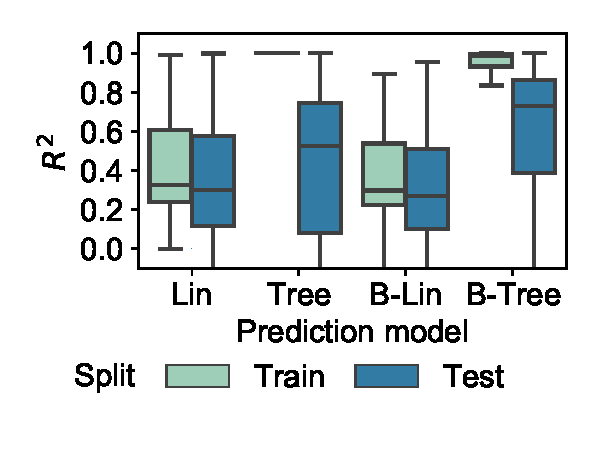
\includegraphics[width=\textwidth, trim=15 25 15 15, clip]{plots/syn-prediction-performance-all.pdf}
		\caption{All experimental runs.}
		\label{fig:syn:prediction-performance-all}
	\end{subfigure}
	\hfill
	\begin{subfigure}{0.48\textwidth}
		\centering
		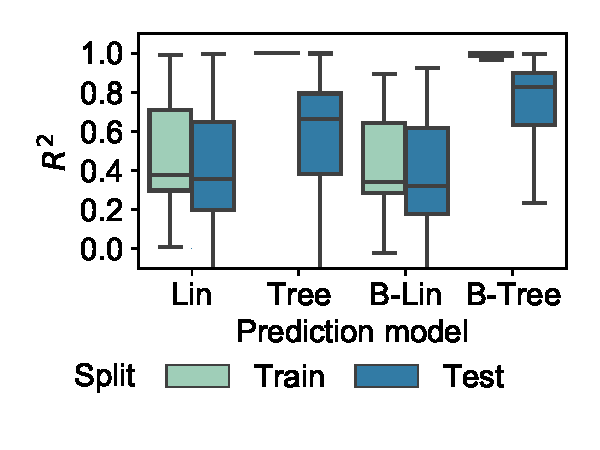
\includegraphics[width=\textwidth, trim=15 25 15 15, clip]{plots/syn-prediction-performance-unconstrained.pdf}
		\caption{Unconstrained experimental runs.}
		\label{fig:syn:prediction-performance-unconstrained}
	\end{subfigure}
	\caption{
		Distribution of prediction performance over datasets, cross-validation folds, and constraint-generation runs, by prediction model.
		Y-axes are truncated and outliers are removed to improve readability.
	}
	\label{fig:syn:prediction-performance}
\end{figure}

\subsection{Comparison of Prediction Models}
\label{sec:syn:evaluation:prediction}

Before studying the impact of constraints, we analyze prediction performance regarding the impact of the prediction model and dataset.
Figure~\ref{fig:syn:prediction-performance-all} shows a considerable variation in prediction performance for each model.
This plot aggregates all experimental runs, i.e., different datasets, cross-validation folds, constraint types, and constraint-generation repetitions.
However, Figure~\ref{fig:syn:prediction-performance-unconstrained} displays that there is still a considerable variation in prediction performance in the unconstrained~\ref{enum:syn:constraint-type:unconstrained} runs.
I.e., the datasets have a substantial impact on prediction performance.
We also see overfitting, i.e., the test-set performance is lower than the training-set performance, particularly for tree-based models.
In the following sections, we focus on test-set performance.
Further, we min-max normalize $R^2$ per dataset, cross-validation fold, and prediction model to focus on the relative impact of constraints, ignoring differences in dataset difficulty and model complexity.
Finally, we limit our analyses to two prediction models:
linear regression (\emph{Lin}), the simplest model we use, and gradient-boosted trees (\emph{B-Tree}), which yield the best average performance.

\begin{figure}[t]
	\centering
	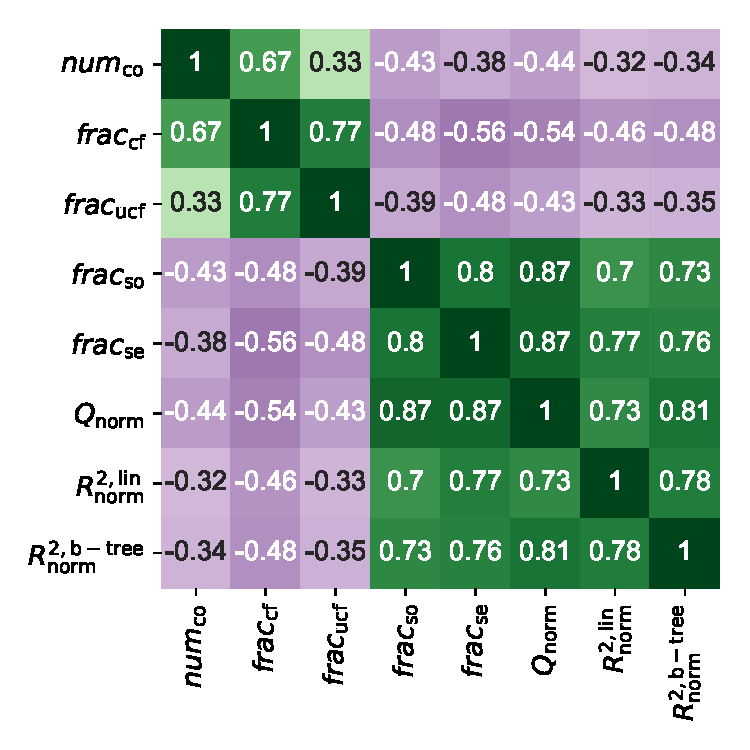
\includegraphics[width=0.66\textwidth, trim=10 10 10 10, clip]{plots/syn-evaluation-metrics-correlation.pdf}
	\caption{Spearman correlation between evaluation metrics, over datasets, cross-validation folds, and constraint-generation runs.}
	\label{fig:syn:evaluation-metrics-correlation}
\end{figure}

\begin{figure}[t]
	\centering
	\begin{subfigure}{0.48\textwidth}
		\centering
		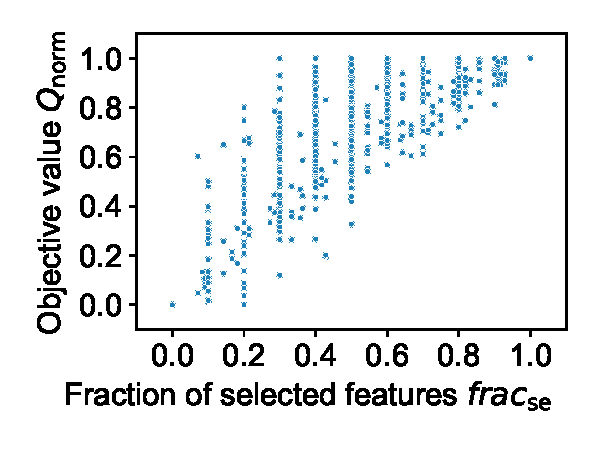
\includegraphics[width=\textwidth, trim=15 15 15 10, clip]{plots/syn-selected-vs-objective.pdf}
		\caption{Fraction of selected features.}
		\label{fig:syn:selected-vs-objective}
	\end{subfigure}
	\hfill
	\begin{subfigure}{0.48\textwidth}
		\centering
		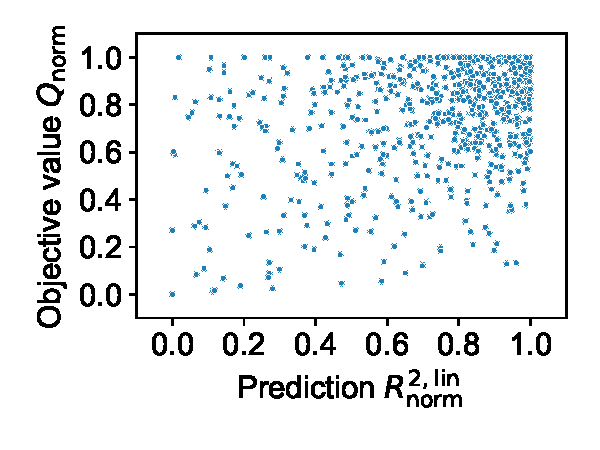
\includegraphics[width=\textwidth, trim=15 15 15 10, clip]{plots/syn-frac-linear-regression-r2-vs-objective.pdf}
		\caption{Test-set prediction performance of linear regression.}
		\label{fig:syn:frac-linear-regression-r2-vs-objective}
	\end{subfigure}
	\\
	\begin{subfigure}{0.48\textwidth}
		\centering
		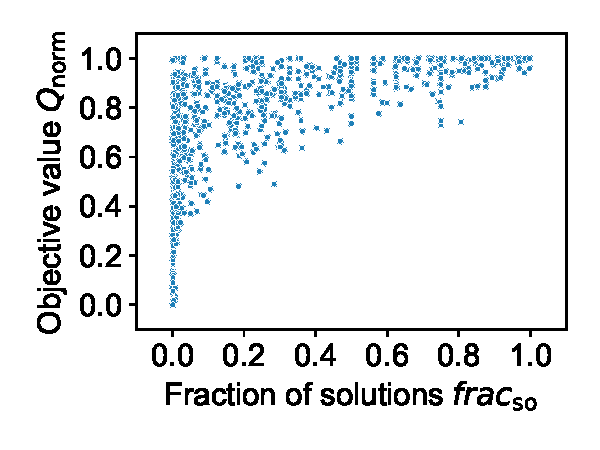
\includegraphics[width=\textwidth, trim=15 15 15 10, clip]{plots/syn-solutions-vs-objective.pdf}
		\caption{Fraction of solutions.}
		\label{fig:syn:solutions-vs-objective}
	\end{subfigure}
	\hfill
	\begin{subfigure}{0.48\textwidth}
		\centering
		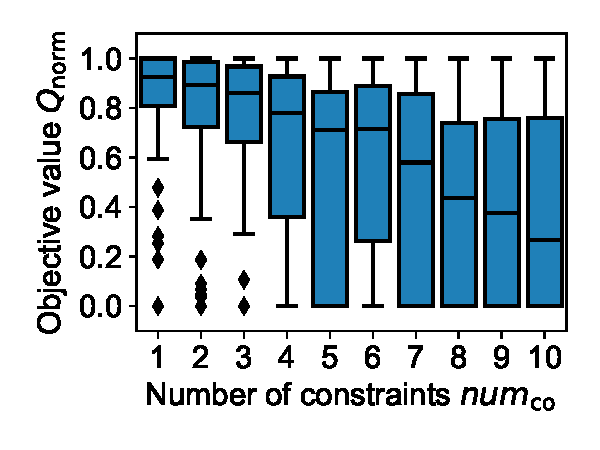
\includegraphics[width=\textwidth, trim=15 15 15 10, clip]{plots/syn-constraints-vs-objective.pdf}
		\caption{Number of constraints.}
		\label{fig:syn:constraints-vs-objective}
	\end{subfigure}
	\caption{
		Relationship of objective value~$Q_{\text{norm}}$ to other evaluation metrics.
		We have randomly sampled 1000 constraint-generation runs to keep the plot sizes and the time for rendering these plots reasonable.
	}
	\label{fig:syn:metrics-vs-metrics}
\end{figure}

\subsection{Relationship Between Evaluation Metrics}
\label{sec:syn:evaluation:metrics}

We study the relationships between evaluation metrics in two ways:
We analyze the correlation between metrics and also plot the metrics against each other.
For the correlation analysis, we take the values of each evaluation metric for all experimental runs and compute the Spearman rank correlation between these vectors.
The resulting correlation matrix (cf.~Figure~\ref{fig:syn:evaluation-metrics-correlation}) shows a strong positive correlation between the fraction of selected features~$\mathit{frac}_{\text{se}}$, the fraction of solutions~$\mathit{frac}_{\text{so}}$, the objective value~$Q_{\text{norm}}$, and the prediction performance~$R^{2}_{\text{norm}}$.
All pairwise correlations between these metrics are at least 0.7.

For a more detailed view, Figure~\ref{fig:syn:selected-vs-objective} shows a roughly linear relationship between the fraction of selected features~$\mathit{frac}_{\text{se}}$ and the objective value~$Q_{\text{norm}}$.
The linear objective function in our experiments (cf.~Section~\ref{sec:syn:experimental-design:objective}) makes this trend plausible.
However, the quality of the selected features and thus the objective value for a fixed feature-set size can still vary since different constraints may exclude different feature combinations.

Figure~\ref{fig:syn:frac-linear-regression-r2-vs-objective} shows that the objective value~$Q_{\text{norm}}$ and the prediction performance~$R^{2}_{\text{norm}}$ may lead to different assessments of feature-set quality.
The chosen objective function cannot describe interactions between features, as it only sums up the individual feature qualities.
This caveat is a general characteristic of univariate filter feature selection.
In contrast, prediction models evaluate a feature set as a whole.

Figure~\ref{fig:syn:solutions-vs-objective} shows that the relationship between the fraction of solutions~$\mathit{frac}_{\text{so}}$ and objective value~$Q_{\text{norm}}$ is non-linear.
Decreasing the fraction of valid feature sets tends to decrease the objective value.
However, it also matters which feature sets become invalid since the optimizer might find feature sets with a high objective value even in small search spaces, depending on the concrete constraints and the distribution of feature qualities.
In contrast, we have not observed any scenario with a large search space but a low objective value.

Coming back to the correlation matrix in Figure~\ref{fig:syn:evaluation-metrics-correlation},
there is a moderately negative correlation between the fraction of solutions~$\mathit{frac}_{\text{so}}$ on the one side and the number of constraints~$\mathit{num}_{\text{co}}$, fraction of constrained features~$\mathit{frac}_{\text{cf}}$, and fraction of unique constrained features~$\mathit{frac}_{\text{ucf}}$ on the other side.
This effect is expected since stronger constraint sets prune more solutions.
The correlation is only moderate, though, since the latter three metrics do not consider the constraint type.
E.g., for \emph{Group-NAND}~\ref{enum:syn:constraint-type:group-nand}, involving more features even makes the constraint weaker.
Further, the latter three metrics only show a moderately negative correlation to feature-set quality since they do not consider the individual feature qualities at all.
For example, Figure~\ref{fig:syn:constraints-vs-objective} shows the high variation in the relationship between the number of constraints~$\mathit{num}_{\text{co}}$ and the objective value~$Q_{\text{norm}}$.

\begin{figure}[t]
	\centering
	\begin{subfigure}{0.48\textwidth}
		\centering
		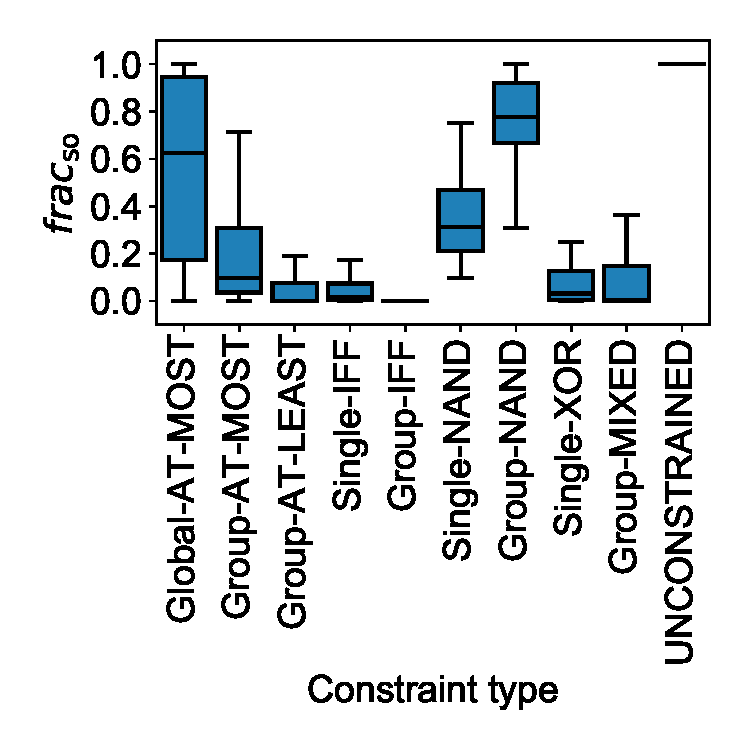
\includegraphics[width=\textwidth, trim=20 15 15 15, clip]{plots/syn-constraint-type-vs-solutions.pdf}
		\caption{Fraction of solutions.}
		\label{fig:syn:constraint-type-vs-solutions}
	\end{subfigure}
	\hfill
	\begin{subfigure}{0.48\textwidth}
		\centering
		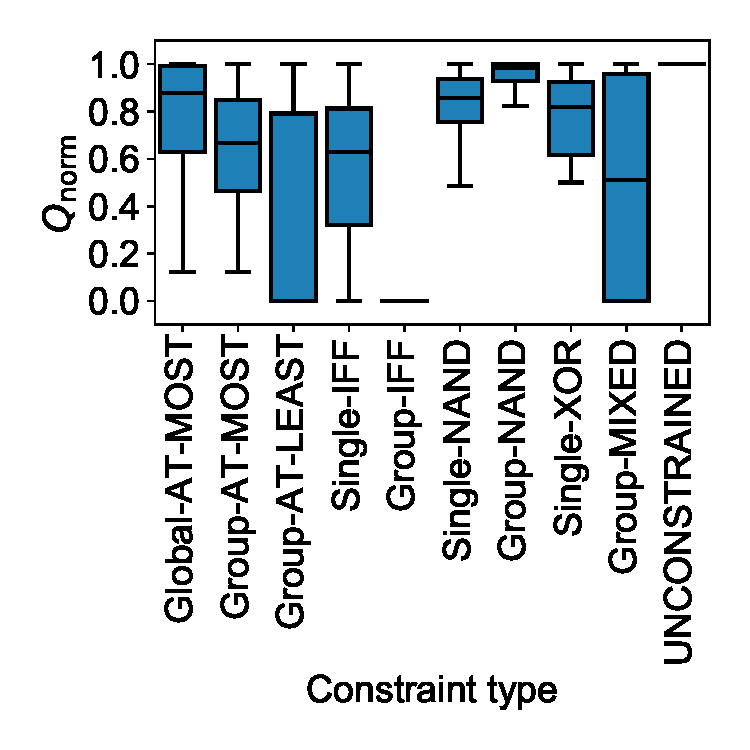
\includegraphics[width=\textwidth, trim=20 15 15 15, clip]{plots/syn-constraint-type-vs-objective.pdf}
		\caption{Objective value.}
		\label{fig:syn:constraint-type-vs-objective}
	\end{subfigure}
	\caption{
		Distribution of evaluation metrics over datasets, cross-validation folds, and constraint-generation runs, by constraint type.
		Outliers are removed to improve readability.
	}
	\label{fig:syn:constraint-type}
\end{figure}

\subsection{Impact of Constraint Types}
\label{sec:syn:evaluation:constraint-types}

Figure~\ref{fig:syn:constraint-type} shows how two evaluation metrics, i.e., fraction of solutions~$\mathit{frac}_{\text{so}}$ and objective value~$Q_{\text{norm}}$, vary between constraint types.
Normalized prediction performance exhibits similar trends as the objective value.
Overall, the impact of constraints strongly depends on the constraint type.
Without constraints, i.e., for the type \emph{UNCONSTRAINED}~\ref{enum:syn:constraint-type:unconstrained}, all feature sets are valid, and the objective value is maximal.
\emph{Global-AT-MOST}~\ref{enum:syn:constraint-type:global-at-most} has the largest inter-quartile range of the fraction of solutions (cf.~Figure~\ref{fig:syn:constraint-type-vs-solutions}).
This effect is expected since we systematically generate only one constraint of this type for each possible feature-set size, while the remaining constraint types employ up to 10 constraints (cf.~Algorithm~\ref{al:syn:constraint-generation}) and thereby typically limit the search space more.
Thus, \emph{GROUP-AT-MOST}~\ref{enum:syn:constraint-type:group-at-most} exhibits a smaller range and lower median of~$\mathit{frac}_{\text{so}}$ than \emph{Global-AT-MOST}~\ref{enum:syn:constraint-type:global-at-most}.
The type \emph{Group-MIXED}~\ref{enum:syn:constraint-type:group-mixed} shows the widest distribution of the objective value (cf.~Figure~\ref{fig:syn:constraint-type-vs-objective}) since it combines different other constraint types.
\emph{Single-NAND}~\ref{enum:syn:constraint-type:single-nand} and \emph{Group-NAND}~\ref{enum:syn:constraint-type:group-nand} exhibit only a small decrease in objective value since \emph{NAND} only excludes selecting all involved features simultaneously.
The more features are involved, the less restrictive the constraint becomes.
In contrast, \emph{IFF}~\ref{enum:syn:constraint-type:single-iff}~\ref{enum:syn:constraint-type:group-iff} constraints become stronger when applied to more features since they require either all of these features to be selected or none.
Further, remember that we combine \emph{IFF} with a \emph{Global-AT-MOST}~\ref{enum:syn:constraint-type:global-at-most} constraint to prevent the trivial outcome of selecting all features.
The more features are involved in \emph{IFF}s, the more difficult it becomes to satisfy the global cardinality constraint.
In the worst case, the set of selected features becomes empty, which is valid but has an objective value of zero.

\subsection{Summary}
\label{sec:syn:evaluation:summary}

We observed a relationship between the size of the search space~$\mathit{frac}_{\text{so}}$ and the feature-set quality, i.e., objective value~$Q_{\text{norm}}$ and prediction performance~$R^{2}_{\text{norm}}$.
Both the fraction of selected features $\mathit{frac}_{\text{se}}$ and the feature-set quality tended to decrease when constraints became stronger, i.e., pruned solutions.
However, the effect was non-linear, i.e., stronger constraints could still yield high feature-set quality.
In particular, there may be sweet spots, i.e., high-quality feature sets that adhere to the constraints.
While feature-set quality was strongly related to the fraction of solutions, the latter is costly to compute.
To a lesser extent, more coarse-grained metrics like the number of constraints~$\mathit{num}_{\text{co}}$ and the fraction of constrained features~$\mathit{frac}_{\text{cf}}$ were also related to feature-set quality.
Further, the distribution of evaluation metrics strongly depended on the constraint type.
Thus, it is difficult to make statements about the impact of constraints apart from some general trends. 
Finally, the optimization's objective value~$Q_{\text{norm}}$ and the prediction performance~$R^{2}_{\text{norm}}$ may yield different values for feature-set quality, particularly if the objective employs a simplified quality criterion like the linear function from Equation~\ref{eq:fs:univariate-filter}.
